\documentclass[12pt]{article}
\usepackage{tikz}
\usepackage{amsmath}
\usepackage{geometry}
\geometry{a4paper, margin=1in}
\usetikzlibrary{arrows.meta, decorations.pathreplacing, positioning}

\tikzset{
	box/.style={draw, thick, minimum size=6mm, inner sep=0pt},
	base/.style={box, fill=blue!20},
	slope/.style={box, fill=red!20},
	overlap/.style={box, fill=purple!40},
	normal/.style={box, fill=gray!10}
}

\begin{document}
	
	\begin{center}
		\LARGE \textbf{Franklin's Involution: Visualizing the Proof}\\
		\large Euler's Pentagonal Number Theorem
	\end{center}
	
	\vspace{0.5cm}
	
	% =================================================================
	% PART 1: The Setup
	% =================================================================
	\section*{1. The Signed Generating Function}
	Expanding $\prod_{k=1}^\infty (1-q^k)$ generates partitions into distinct parts. A partition into an even number of parts contributes $+1$, and an odd number of parts contributes $-1$.
	
	\begin{center}
		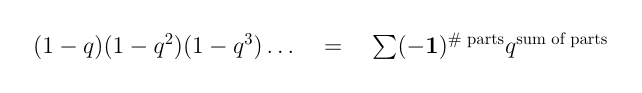
\begin{tikzpicture}[scale=0.6, transform shape]
			\node[right, font=\Large] at (-2, 1) {$(1-q)(1-q^2)(1-q^3)\dots \quad = \quad \sum (\mathbf{-1})^{\text{\# parts}} q^{\text{sum of parts}}$};
		\end{tikzpicture}
	\end{center}
	
	\vspace{0.5cm}
	
	% =================================================================
	% PART 2: The Involution
	% =================================================================
	\section*{2. The Sign-Reversing Involution}
	We pair almost all partitions by moving the \textbf{Base $b$} (blue) to the \textbf{Slope $s$} (red), or vice versa, whichever is smaller. This adds or removes exactly one part, flipping the sign and causing them to cancel in the sum.
	
	\vspace{0.5cm}
	\begin{center}
		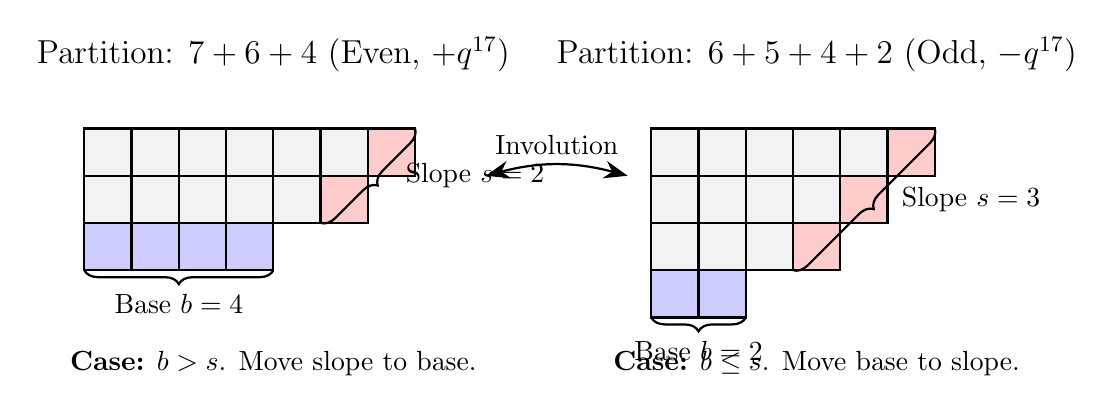
\begin{tikzpicture}[scale=0.6]
			% --- Left Diagram: 7 + 6 + 4 ---
			\begin{scope}[shift={(0,0)}]
				\node[above, font=\large] at (3.5, 3.5) {Partition: $7+6+4$ (Even, $+q^{17}$)};
				
				% Row 1 (7)
				\foreach \x in {0,1,2,3,4,5} \node[normal] at (\x, 2) {};
				\node[slope] at (6, 2) {};
				% Row 2 (6)
				\foreach \x in {0,1,2,3,4} \node[normal] at (\x, 1) {};
				\node[slope] at (5, 1) {};
				% Row 3 (4)
				\foreach \x in {0,1,2,3} \node[base] at (\x, 0) {};
				
				% Labels
				\draw[decorate,decoration={brace,amplitude=5pt,mirror},thick] (-0.5,-0.5) -- (3.5,-0.5) node[midway,below=5pt] {Base $b=4$};
				\draw[decorate,decoration={brace,amplitude=5pt},thick] (6.5,2.5) -- (4.5,0.5) node[midway,right=10pt] {Slope $s=2$};
				
				\node[below, font=\normalsize] at (3.5, -2) {\textbf{Case:} $b > s$. Move slope to base.};
			\end{scope}
			
			% --- Arrows ---
			\draw[{Stealth[length=3mm]}-{Stealth[length=3mm]}, thick, bend left=15] (8, 1.5) to node[above] {Involution} (11, 1.5);
			
			% --- Right Diagram: 6 + 5 + 4 + 2 ---
			\begin{scope}[shift={(12,0)}]
				\node[above, font=\large] at (3, 3.5) {Partition: $6+5+4+2$ (Odd, $-q^{17}$)};
				
				% Row 1 (6)
				\foreach \x in {0,1,2,3,4} \node[normal] at (\x, 2) {};
				\node[slope] at (5, 2) {};
				% Row 2 (5)
				\foreach \x in {0,1,2,3} \node[normal] at (\x, 1) {};
				\node[slope] at (4, 1) {};
				% Row 3 (4)
				\foreach \x in {0,1,2} \node[normal] at (\x, 0) {};
				\node[slope] at (3, 0) {};
				% Row 4 (2)
				\foreach \x in {0,1} \node[base] at (\x, -1) {};
				
				% Labels
				\draw[decorate,decoration={brace,amplitude=5pt,mirror},thick] (-0.5,-1.5) -- (1.5,-1.5) node[midway,below=5pt] {Base $b=2$};
				\draw[decorate,decoration={brace,amplitude=5pt},thick] (5.5,2.5) -- (2.5,-0.5) node[midway,right=10pt] {Slope $s=3$};
				
				\node[below, font=\normalsize] at (3, -2) {\textbf{Case:} $b \le s$. Move base to slope.};
			\end{scope}
		\end{tikzpicture}
	\end{center}
	
	\vspace{0.5cm}
	
	% =================================================================
	% PART 3: The Exceptions
	% =================================================================
	\section*{3. The Unpaired Partitions (Pentagonal Numbers)}
	The involution fails exactly when the base and slope intersect, making it impossible to move the blocks without violating the "distinct parts" rule or creating an invalid shape. This happens in exactly two structural cases for each $k$.
	
	\vspace{0.5cm}
	\begin{center}
		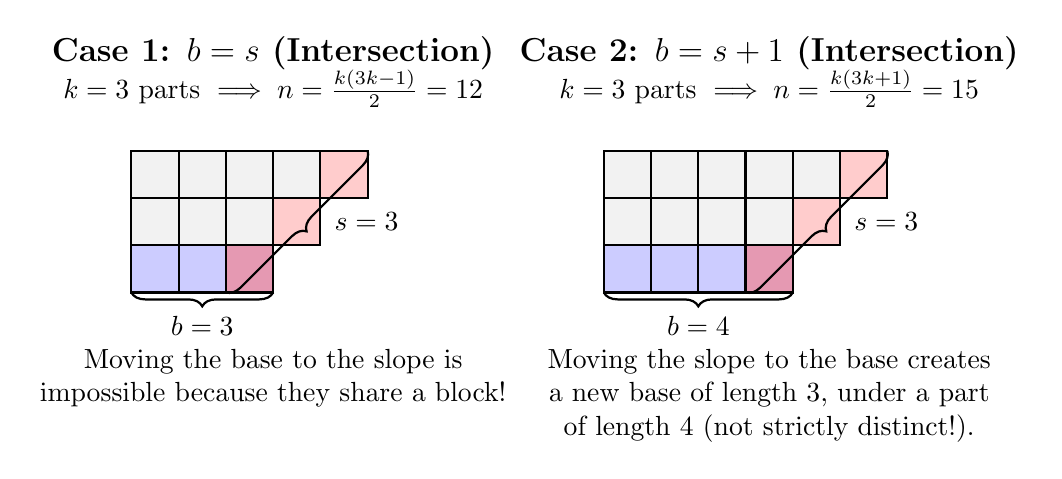
\begin{tikzpicture}[scale=0.6]
			% --- Exception 1 ---
			\begin{scope}[shift={(0,0)}]
				\node[above, font=\large] at (2.5, 3.5) {\textbf{Case 1: $b = s$ (Intersection)}};
				\node[above, font=\normalsize] at (2.5, 2.7) {$k=3$ parts $\implies n = \frac{k(3k-1)}{2} = 12$};
				
				% Row 1 (5)
				\foreach \x in {0,1,2,3} \node[normal] at (\x, 1.5) {};
				\node[slope] at (4, 1.5) {};
				% Row 2 (4)
				\foreach \x in {0,1,2} \node[normal] at (\x, 0.5) {};
				\node[slope] at (3, 0.5) {};
				% Row 3 (3)
				\node[base] at (0, -0.5) {};
				\node[base] at (1, -0.5) {};
				\node[overlap] at (2, -0.5) {}; % Overlap
				
				% Labels
				\draw[decorate,decoration={brace,amplitude=5pt,mirror},thick] (-0.5,-1) -- (2.5,-1) node[midway,below=5pt] {$b=3$};
				\draw[decorate,decoration={brace,amplitude=5pt},thick] (4.5,2) -- (1.5,-1) node[midway,right=10pt] {$s=3$};
				
				\node[below, font=\normalsize, text width=6cm, align=center] at (2.5, -2) {Moving the base to the slope is impossible because they share a block!};
			\end{scope}
			
			% --- Exception 2 ---
			\begin{scope}[shift={(10,0)}]
				\node[above, font=\large] at (3, 3.5) {\textbf{Case 2: $b = s + 1$ (Intersection)}};
				\node[above, font=\normalsize] at (3, 2.7) {$k=3$ parts $\implies n = \frac{k(3k+1)}{2} = 15$};
				
				% Row 1 (6)
				\foreach \x in {0,1,2,3,4} \node[normal] at (\x, 1.5) {};
				\node[slope] at (5, 1.5) {};
				% Row 2 (5)
				\foreach \x in {0,1,2,3} \node[normal] at (\x, 0.5) {};
				\node[slope] at (4, 0.5) {};
				% Row 3 (4)
				\node[base] at (0, -0.5) {};
				\node[base] at (1, -0.5) {};
				\node[base] at (2, -0.5) {};
				\node[overlap] at (3, -0.5) {}; % Overlap
				
				% Labels
				\draw[decorate,decoration={brace,amplitude=5pt,mirror},thick] (-0.5,-1) -- (3.5,-1) node[midway,below=5pt] {$b=4$};
				\draw[decorate,decoration={brace,amplitude=5pt},thick] (5.5,2) -- (2.5,-1) node[midway,right=10pt] {$s=3$};
				
				\node[below, font=\normalsize, text width=6.5cm, align=center] at (3, -2) {Moving the slope to the base creates a new base of length 3, under a part of length 4 (not strictly distinct!).};
			\end{scope}
		\end{tikzpicture}
	\end{center}
	
\end{document}